\documentclass[12pt,a4paper]{book}
\usepackage[utf8]{inputenc}
\usepackage[spanish]{babel}
\usepackage{graphicx}
\usepackage{color}
\usepackage{fancyhdr}
\usepackage[left=2cm,right=2cm,top=2cm,bottom=2cm]{geometry}
\author{Felipe de Jesus Ruiz Garcia}
\title{Metodos Matematicos 2 : Actividad 1}
\pagestyle{fancy}
\newcommand{\setFooterR}[1]{
    \fancyfoot[R]{\small\textit{#1}}
}
\setFooterR{\textbf{TRABAJO REALIZADO EN \LaTeX}}

\begin{document}
\begin{figure}[hbtp]
\centering

\includegraphics[scale=.5]{../PRE/udg.png}\\
 \textbf{Universidad de Guadalajara}
\end{figure}

\begin{center}
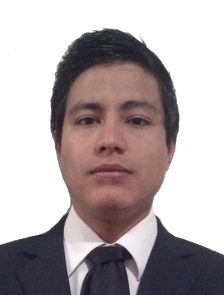
\includegraphics[scale=.5]{../PRE/profile.png}\\
\end{center}

\begin{center}
\textbf{TAREA : SINTESIS DEL M201 \\}
\textbf{FECHA : 14 FEB 2017 23:59:59 \\}

Felipe de Jesus Ruiz Garcia 
\\ 214522077
\\ Grupo F  
\\ Maestro :  Jose Manuel Jimenez Mora

\end{center}
 \bigskip

\begin{figure}[hbtp]
\centering

\end{figure}
\begin{center}
\end{center}


\newpage

\section{Péndulo invertido}
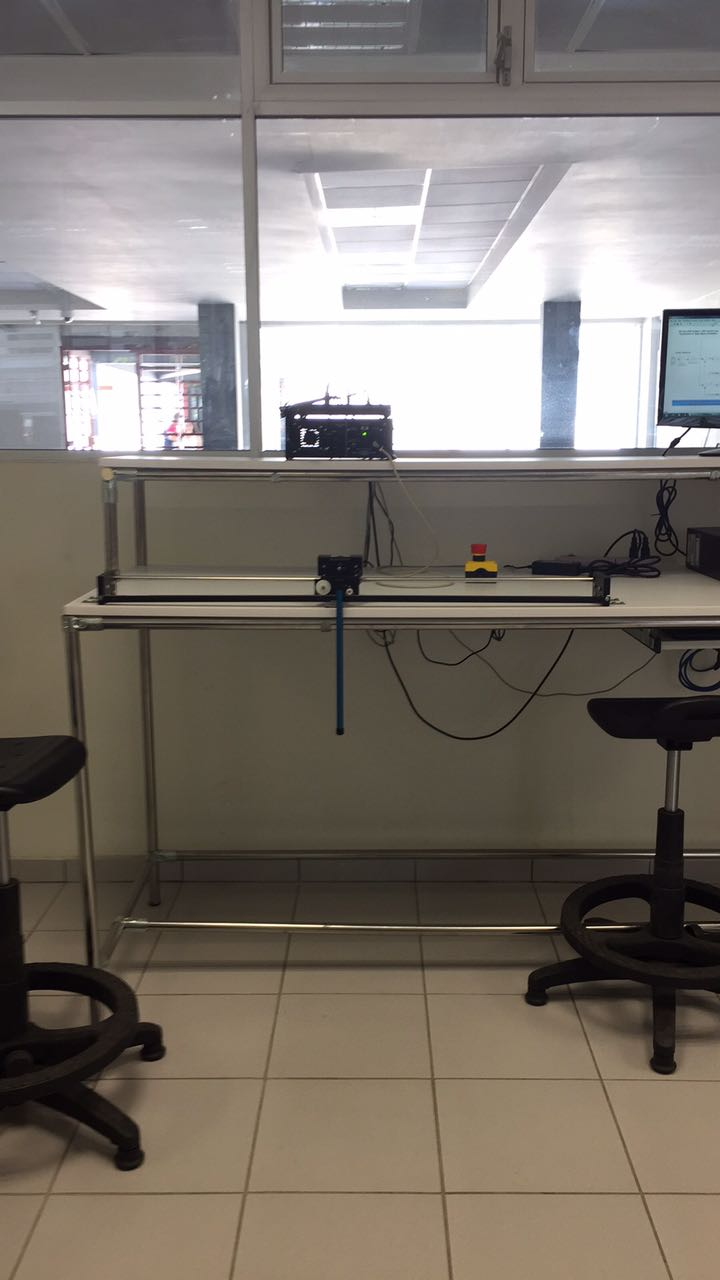
\includegraphics[scale=.25]{./1.jpeg}
\\ El péndulo invertido es un servo mecanismo que consta de un riel sobre
el cual se puede deslizar un carro, montado un péndulo que
puede girar libremente. 
\\
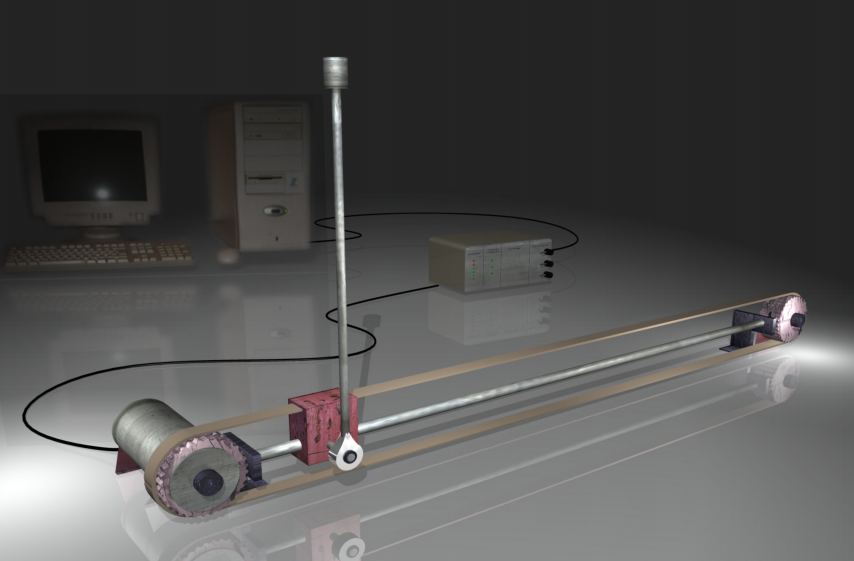
\includegraphics[scale=.4]{./1_pendulo.png}
\\
El sistema esta instrumentado, de tal suerte que
se puede medir el angulo del péndulo con respecto a la vertical, así como
la posición y la velocidad del carro. A través de un motor y una banda
conectada al carro, se puede hacer que este se deslice sobre el riel, el cual
mide aproximadamente 1.2m. \\

\newpage
\section{Tanques acoplados}
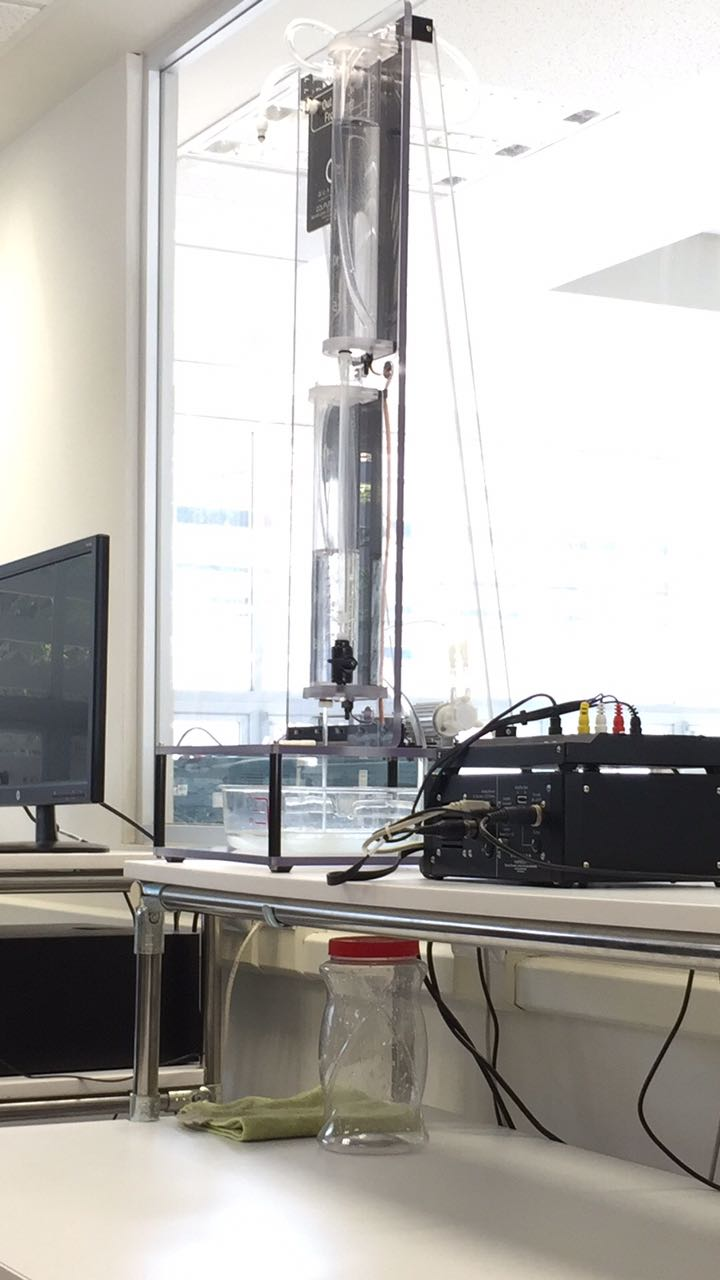
\includegraphics[scale=.25]{./2.jpeg}

Este sistema, a través de un sensor de presión, puede mantener el nivel de agua en cierto rango tomando en cuenta una fuga con flujo variable.
\\
Los 2 tanques dispuestos en el frente del panel están configurados de manera que la salida de agua del primer tanque caiga en el segundo y la salida de este caiga en el recipiente principal.
\\
\\ 
El caudal de salida en ambos tanques puede modificarse mediante cambio en los diámetros de los orificios de los pasadores que se coloca en los huecos roscados.
\\
Se suministra las tuberías plásticas con acoplamientos apropiados para permitir que la bomba alimente uno o ambos tanques.
\\
La selección de salida de la bomba controla la relación de flujo de ambos tanques.
\\
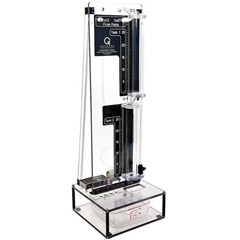
\includegraphics[scale=1]{./2_tanques_acoplados.jpg}


\newpage
\section{Levitación magnética}
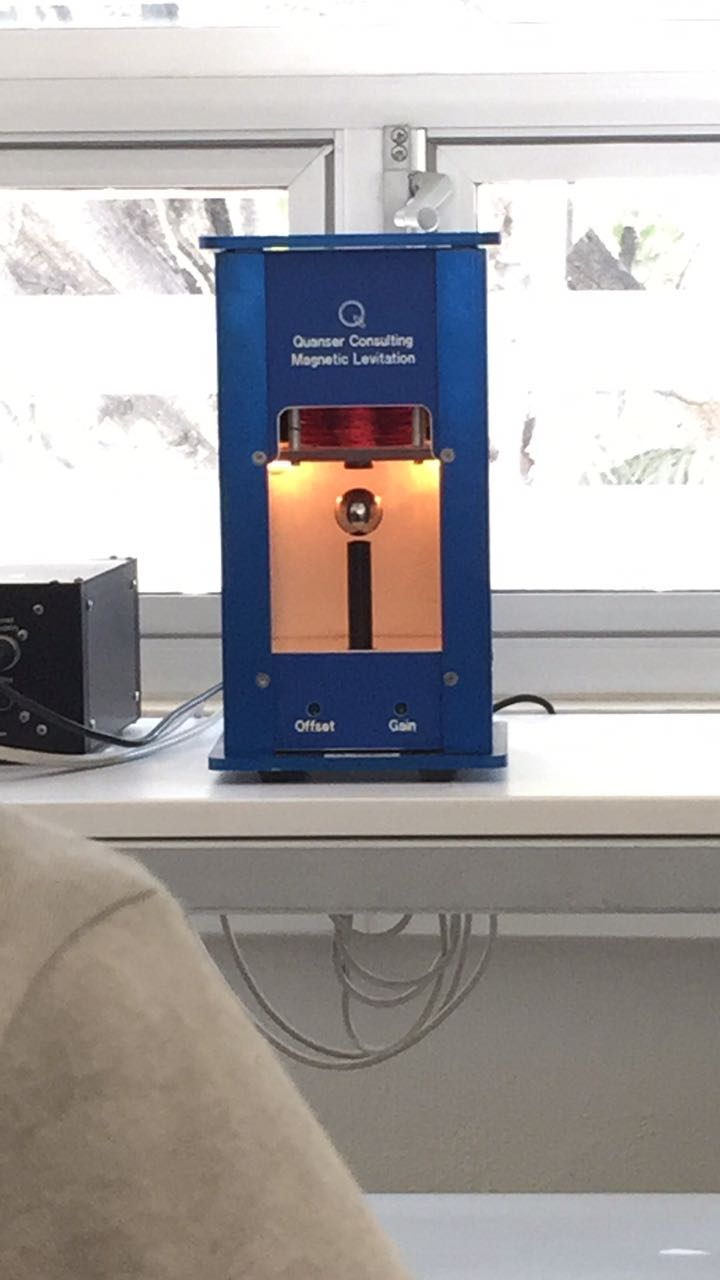
\includegraphics[scale=.25]{./3.jpeg}
\\
\\
La Levitación Magnética es un sistema de suspensión electromagnética que actúa sobre una bola de acero. El electro imán, situado en la parte superior del dispositivo, es capaz de levantar la bola de acero desde su pedestal y mantenerla en el espacio libre, haciendo parecer que ni la gravedad es ley.
\\
Uno de los polos de electro imán está orientado hacia la parte superior de un poste en el que descansa la bola.\\
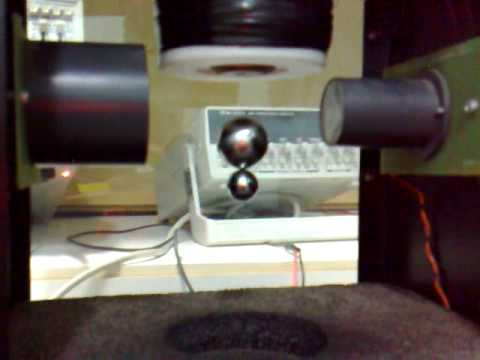
\includegraphics[scale=1]{./3_image.jpeg}
\\
La elevación de la bola desde la parte superior del poste se mide usando un sensor.\\
\newpage
\section{Bola y viga}
EL sistema consiste en el control de una bola de acero rodando sobre barras metálicas montadas sobre un eje de un motor eléctrico. La barra se inclina para estabilizar la bola. 
\\
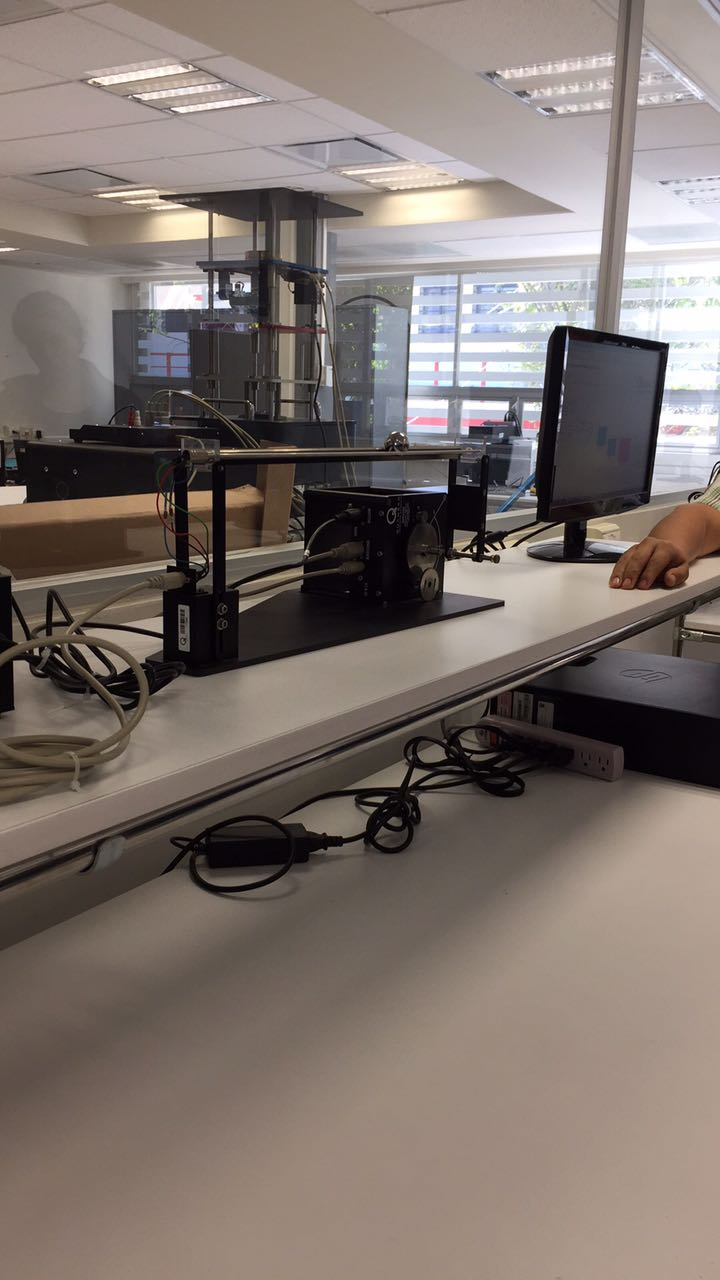
\includegraphics[scale=.25]{./4.jpeg}

\newpage
\section{Péndulo de rotación}
Es muy similar a el péndulo invertido, a diferencia este, no esta limitado del movimiento del carro donde se monta el péndulo, sin embargo, esta apoyado sobre un brazo ; lo cual le permite rotar y no desplazare.
\\
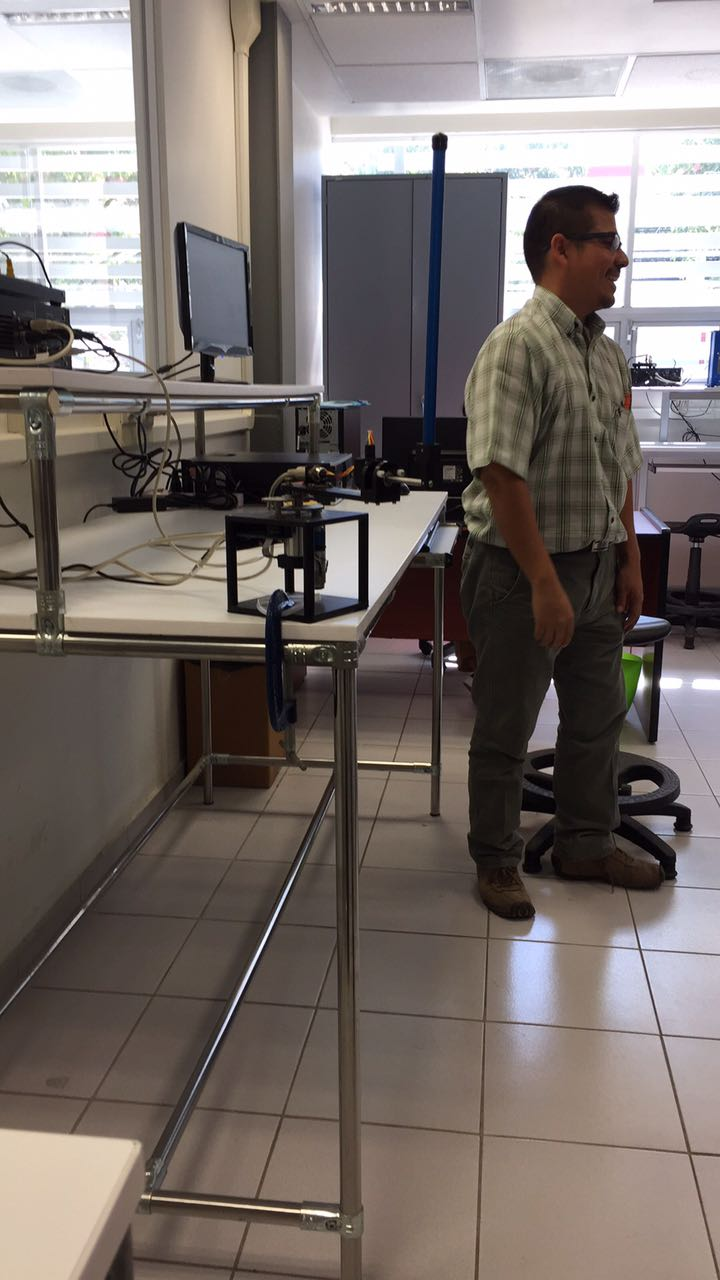
\includegraphics[scale=.25]{./5.jpeg}

\end{document}